\chapter{Aeroelastic study} \label{chap:aeroelastic}

  %Intro
  In the present chapter, the compliant design for the wing-box is embedded into a full wing model. A pressure field is then introduced to simulated the pressure distribution obtained from the evaluation of the aerodynamic forces around the airfoil.

  \section{Wing model} \label{sec:wingModel_aeroelastic}

    The wing model is described in the present section. Firstly, the airfoil is one standard NACA 0012 and the chord is constant throughout the whole span. The wing geometrical characterization is completed by the span $s$, the chord length $c_0$, and the position of the front and rear spars of the wing-box, $c_1$ and $c_2$, respectively and in the chordwise direction. These two last parameters are expressed in dimensionless form as a function of $c_0$, resulting on $\hat{c}_1 = c_1 /c_0$ for the front spar and in $\hat{c}_2 = c_2 /c_0$ for the rear spar. The computational model built only comprises half of the span. This geometrical description of the wing is also graphically shown in Figure \ref{fig:wing-dim}. 

    \begin{figure}[!htpb]
      \centering
      \subfigure[Airfoil dimensions.]{\label{fig:wing-dim1}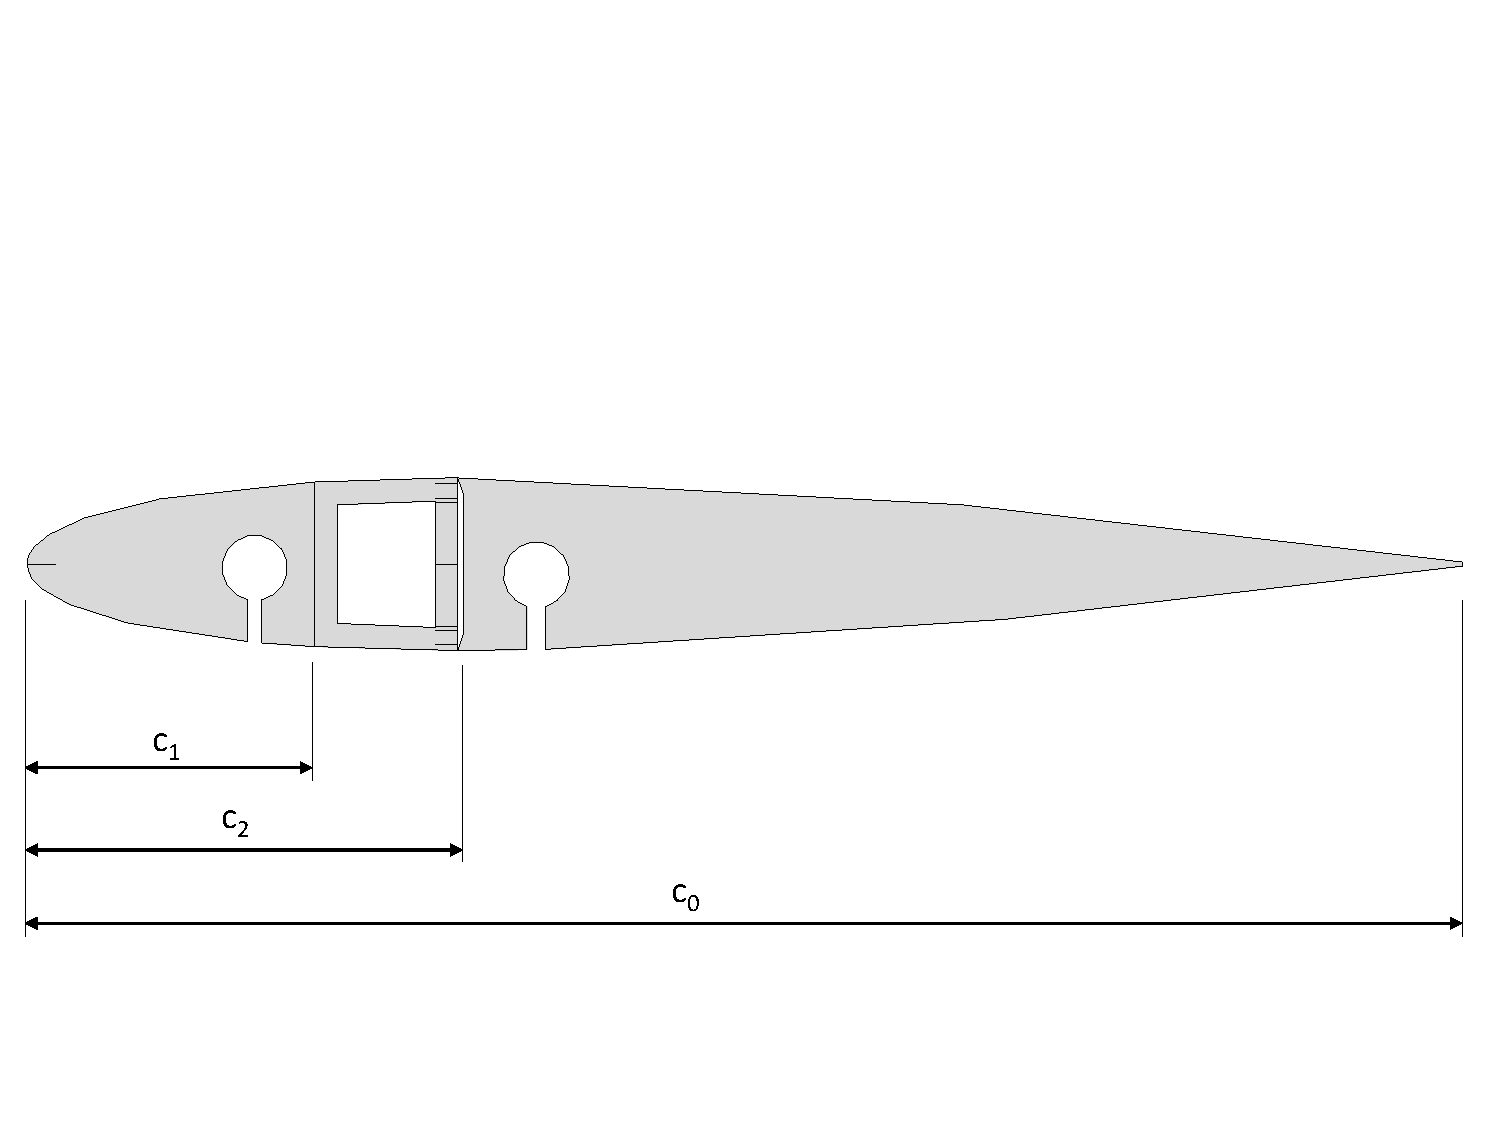
\includegraphics[width=0.6\textwidth]{figures/wing-model/airfoilDim1}} \qquad
      \subfigure[Wing span.]{\label{fig:wing-dim2}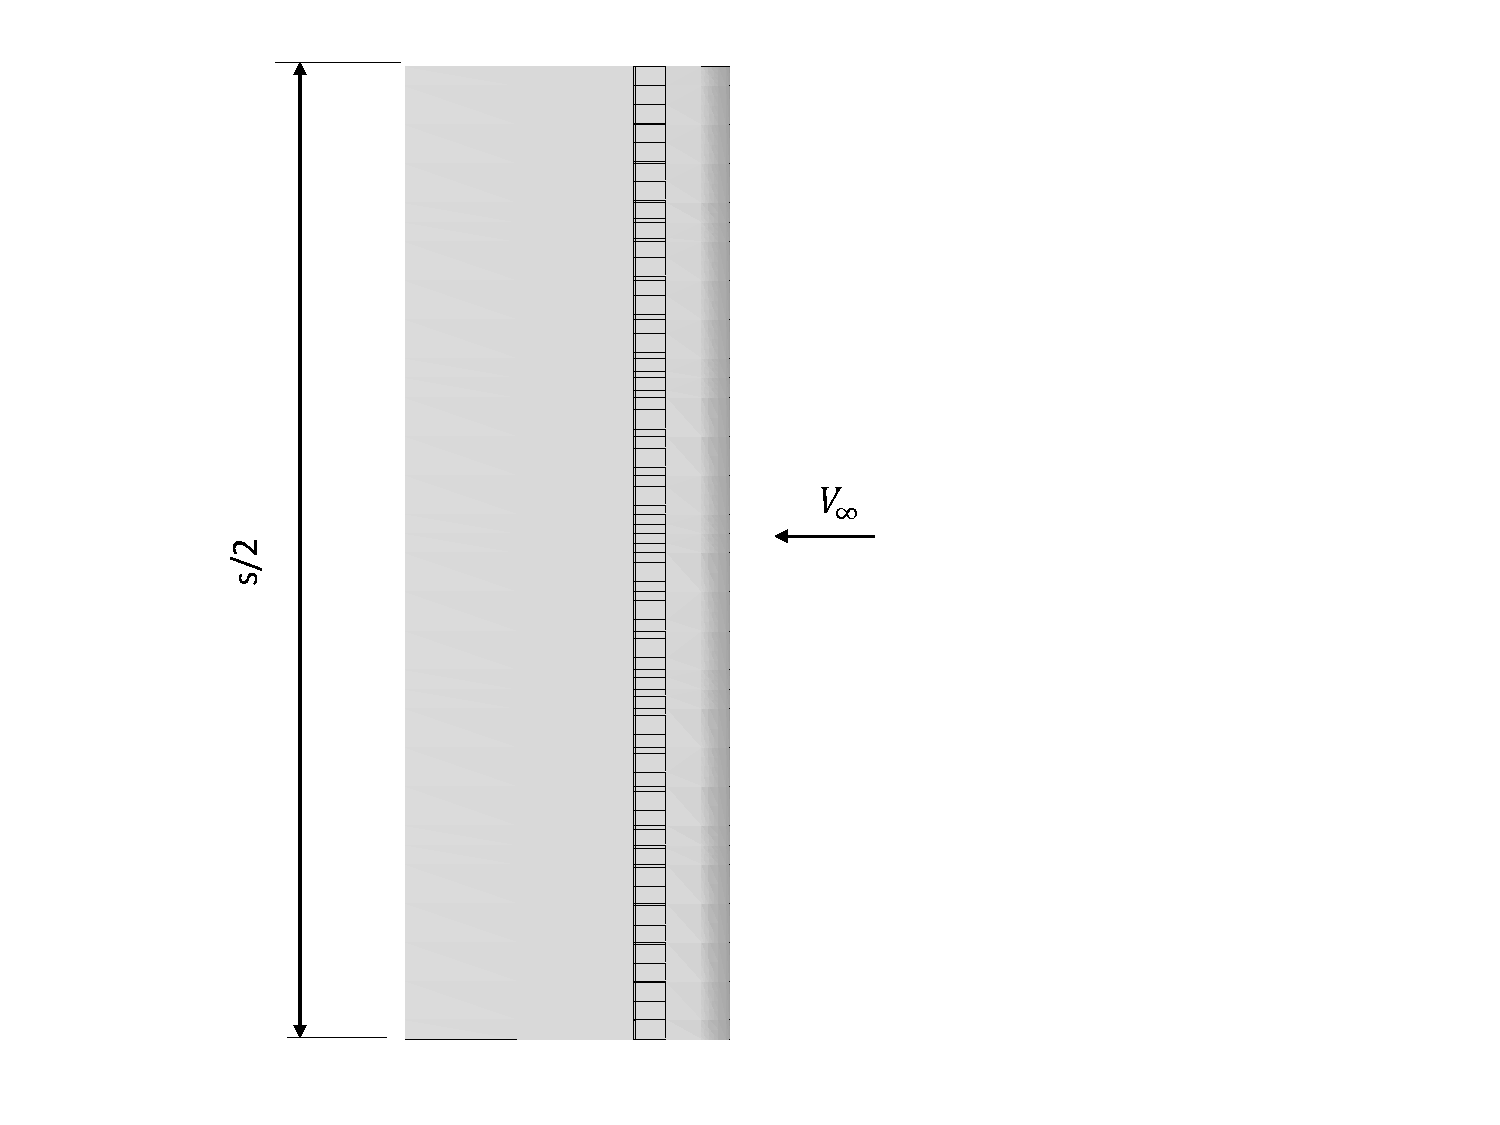
\includegraphics[width=0.3\textwidth]{figures/wing-model/airfoilDim2}}
      \caption[Wing geometrical characterization]{Wing and airfoil geometrical characterization. The airfoil is standard NACA 0012. The parameters are the span $s$, the chord length $c_0$, and the position of the front and rear spars of the wing-box, $c_1$ and $c_2$, respectively.}
      \label{fig:wing-dim}
    \end{figure}

    An overview of the computational model is shown in Figure \ref{fig:wing}. The boundary condition for wing is established using the wing-box which has all its degrees of freedom restrained at the root.

    \begin{figure}[!htpb]
      \centering
      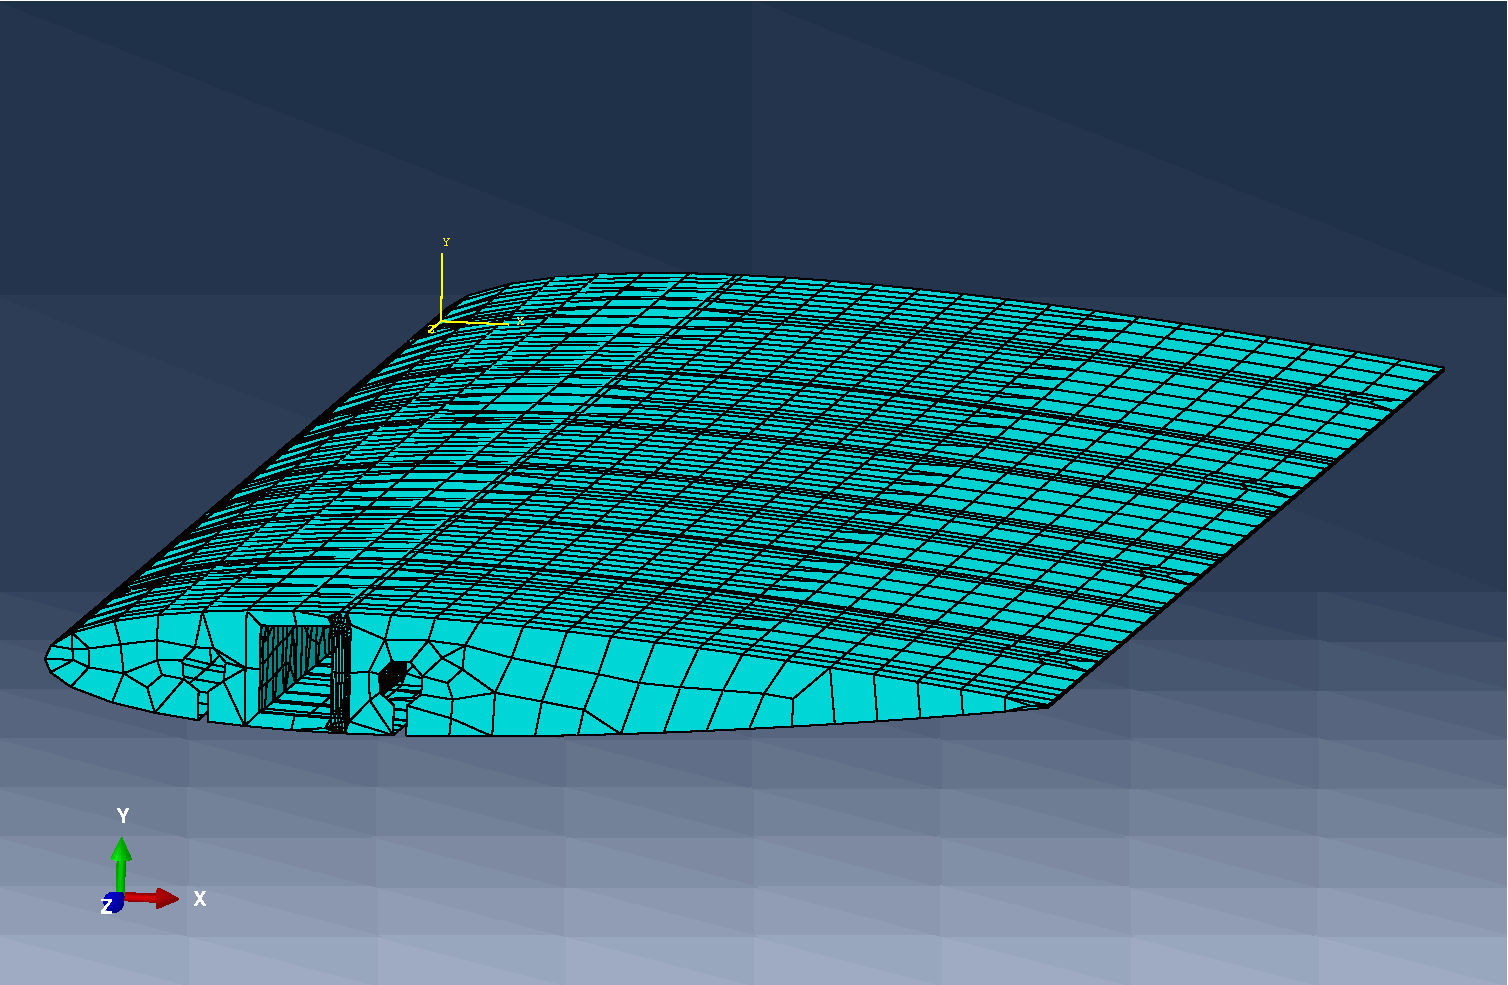
\includegraphics[width=0.7 \textwidth]{figures/wing-model/wing}
      \caption[Overview of the wing FEM model embedded with the compliant wing-box design]{Overview of the wing FEM model embedded with the compliant wing-box design.}
      \label{fig:wing}
    \end{figure}

  \section{Aerodynamic model} \label{sec:aerodynamic_aeroelastic}

    The pressure distribution originated from the fluid-airfoil interaction is responsible of the forces applied into the wing model. This is the only source of forces introduced into the model. The pressure distribution is obtained using \copyright XFOIL software which considers the airfoil geometry and the flight condition.

    The flight condition is determined by introducing the air velocity $V$, the air density $\rho$, the air dynamic viscosity $\mu$

  \section{Weakly coupled static aeroelastic analysis} \label{sec:aeroelastic_aeroelastic}
    % Parameters utilized
    % Desciption of the method

    \begin{table}[!htpb]
    \centering
    \begin{tabular}{|l|lll|}
    \hline
    \textbf{Parameter} & \multicolumn{1}{l|}{\textbf{Symbol}} & \multicolumn{1}{l|}{\textbf{Units}} & \textbf{Nominal value} \\ \hline \hline
    {\textbf{Wing and airfoil dimensions}} &  &  &  \\ \hline
    Span & \multicolumn{1}{l|}{$s$} & \multicolumn{1}{l|}{m} & 3 \\ \hline
    Chord length & \multicolumn{1}{l|}{$c_0$} & \multicolumn{1}{l|}{m} & 0.5 \\ \hline
    Dimensionless position of the front wing-box spar & \multicolumn{1}{l|}{$\hat{c}_1$} & \multicolumn{1}{l|}{} & 0.2 \\ \hline
    Dimensionless position of the rear wing-box spar & \multicolumn{1}{l|}{$\hat{c}_2$} & \multicolumn{1}{l|}{} & 0.3 \\ \hline \hline
    {\textbf{Compliant spar design with lattice of chiral structures}} &  &  &  \\ \hline
    Number of unit cells in spanwise direction & \multicolumn{1}{l|}{$N$} & \multicolumn{1}{l|}{} & 52 \\ \hline
    Number of unit cells in transversal direction & \multicolumn{1}{l|}{$M$} & \multicolumn{1}{l|}{} & 2 \\ \hline
    Dimensionless ligament eccentricity (e/B) & \multicolumn{1}{l|}{$\epsilon_{\mathrm{chi}}$} & \multicolumn{1}{l|}{} & 0.01 \\ \hline
    Node radius & \multicolumn{1}{l|}{$r_{\mathrm{chi}}$} & \multicolumn{1}{l|}{mm} & 2.5355 \\ \hline
    Node depth & \multicolumn{1}{l|}{$B_{\mathrm{chi}}$} & \multicolumn{1}{l|}{mm} & 8 \\ \hline
    Ligament half length & \multicolumn{1}{l|}{$L_{\mathrm{chi}}$} & \multicolumn{1}{l|}{mm} & 14.486 \\ \hline
    Thickness & \multicolumn{1}{l|}{$t_{\mathrm{chi}}$} & \multicolumn{1}{l|}{mm} & 0.4 \\ \hline \hline
    {\textbf{Flight condition}} &  &  &  \\ \hline
    Free-stream air speed & \multicolumn{1}{l|}{$V$} & \multicolumn{1}{l|}{m/s} & 50 \\ \hline
    Angle of attack of the wing & \multicolumn{1}{l|}{$\alpha_0$} & \multicolumn{1}{l|}{deg} & 8 \\ \hline
    Air density & \multicolumn{1}{l|}{$\rho$} & \multicolumn{1}{l|}{kg/m$^3$} & 50 \\ \hline
    Air dynamic viscosity & \multicolumn{1}{l|}{$\mu$} & \multicolumn{1}{l|}{N s/m$^2$} & \notcien{1.789}{-5} \\ \hline
    Air dynamic viscosity & \multicolumn{1}{l|}{$\mu$} & \multicolumn{1}{l|}{N s/m$^2$} & \notcien{1.789}{-5} \\ \hline
    \end{tabular}
    \caption[Parameters that define the aeroelastic analysis]{Parameters that define the aeroelastic analysis. The table includes the wing and airfoil geometrical dimensions, the internal parameter for the lattice of chiral structures and the flight condition.}
    \label{tab:parameters_aeroelastic}
    \end{table}

